%Master File:lectures.tex

\lesson{Declare your intentions (not your actions)}
\vspace*{-2cm}
\begin{center}
    \includegraphics[height=11cm]{declaration}
\end{center}
\vspace*{-1cm}
\keywords{ADTs, stacks, queues, priority queues, sets, maps}

%%%%%%%%%%%%%%%%%%%%%%% Next Slide %%%%%%%%%%%%%%%%%%%%%%%

\renewcommand{\Outline}{%
\begin{slide}
\section{Outline}
\begin{minipage}{10cm}
  \vfill
  \begin{enumerate}\raggedright
    \outlineitem{Abstract Data Types (ADTs)}{adt}
    \outlineitem{Stacks}{stack}
    \outlineitem{Queues and Priority Queues}{queues}
    \outlineitem{Lists, Sets and Maps}{sets}
    \outlineitem{Putting it Together}{together}
  \end{enumerate}
  \vfill
\end{minipage}\hfill
\begin{minipage}{10cm}
  \includegraphics[width=10cm]{declaration}
\end{minipage}
\end{slide}
\addtocounter{outlineitem}{1}
}

\setcounter{outlineitem}{1}
\Outline
\toptarget{firstoutline}

%%%%%%%%%%%%%%%%%%%%%%% Next Slide %%%%%%%%%%%%%%%%%%%%%%%


\begin{slide}
\section{Object Oriented Programming}

\begin{PauseHighLight}
  \begin{itemize}
  \item OO-programming allows you to build large systems reliably\pause
  \item In the OO-methodology you separate the interface from the
    implementation\pause
  \item The \emph{interface} is the public methods (functions) of a class\pause
  \item The implementation is hidden (\emph{encapsulated}) and may be changed
    without affecting how the class is used\pause
  \item There exist other ways of programming, but C++ is designed to
    support the OO-methodology\pause---for building systems it is
    brilliant\pauseb
  \end{itemize}  
\end{PauseHighLight}
\end{slide}

%%%%%%%%%%%%%%%%%%%%%%% Next Slide %%%%%%%%%%%%%%%%%%%%%%%

\begin{slide}
\section{Object-Oriented Classes}

\begin{center}
  \includegraphics[width=\textwidth]{interface}
\end{center}

\end{slide}


%%%%%%%%%%%%%%%%%%%%%%% Next Slide %%%%%%%%%%%%%%%%%%%%%%%

\begin{slide}
\section{Abstract Data Types}

\begin{PauseHighLight}
  \begin{itemize}
  \item With data structures there are some traditional interfaces
    called \emph{Abstract Data Types} or ADTs\pause
  \item These are implementation free data structures\pause
  \item They are mathematical abstractions of the data structure\pause
  \item Their purpose is to allow you to declare you intentions\pause
  \item You are entering into an agreement that you only intend to use
    the underlying data structure in the way specified by the
    interface\pause
  \end{itemize}
\end{PauseHighLight}
\end{slide}

%%%%%%%%%%%%%%%%%%%%%%% Next Slide %%%%%%%%%%%%%%%%%%%%%%%

\begin{slide}
\section{ADTs}

\begin{center}
  \includegraphics[width=\textwidth]{adt}
\end{center}
\end{slide}


%%%%%%%%%%%%%%%%%%%%%%% Next Slide %%%%%%%%%%%%%%%%%%%%%%%

\begin{slide}
\section{Say it with an ADT}

\begin{PauseHighLight}
 \begin{itemize}
 \item Common ADTs include stacks, queues, priority queues,
   sets, multisets and maps\pause
 \item There are many possible implementations of these ADTs\pause\ (some
   far from obvious)\pause
 \item Each ADT has a limited set of methods associated with it\pause
 \item They are an abstraction away from the implementation\pause
 \item By declaring your intentions you are making your code easier to
   understand and maintain\pause
\end{itemize} 
\end{PauseHighLight}
\end{slide}


%%%%%%%%%%%%%%%%%%%%%%% Next Slide %%%%%%%%%%%%%%%%%%%%%%%
\Outline
%%%%%%%%%%%%%%%%%%%%%%% Next Slide %%%%%%%%%%%%%%%%%%%%%%%


\begin{slide}
\section{Stacks}

\pausebuild
\begin{minipage}{14cm}
  \begin{itemize}
    \pauselevel{=1}
  \item Last In First Out (LIFO) memory\pause
  \item Standard functions\pause
  \begin{itemize}
  \item \jl$push(item)$\pause
  \item \jl$T top()$\pause
  \item \jl$T pop()$\pause\pause{} except in C++ \jl$pop()$ doesn't return
    the top of the stack\pause
  \item \jl$boolean empty()$\pause
  \end{itemize}
\item Implemented using an array\pause\ (or a linked-list)\pause
\end{itemize}

\end{minipage}
\hspace*{0.9cm}
\begin{minipage}{9cm}\setlength{\unitlength}{1mm}
  \begin{picture}(90,120)
    \pause\pauselevel{=1 :2}
    \put(0,0){\makebox(90,120)[br]{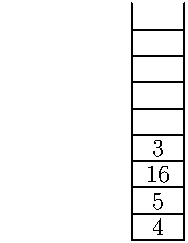
\includegraphics[height=12cm]{stack}}}
    \pause\pauselevel{=3 :3}
    \put(0,0){\makebox(90,120)[br]{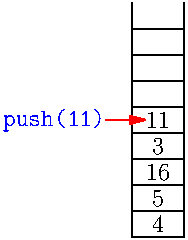
\includegraphics[height=12cm]{stack_push}}}
    \pause \pauselevel{=4 :4}
    \put(0,0){\makebox(90,120)[br]{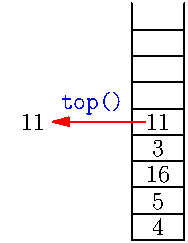
\includegraphics[height=12cm]{stack_top}}}
    \pause\pauselevel{=5 :5}
    \put(0,0){\makebox(90,120)[br]{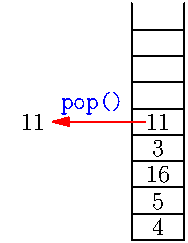
\includegraphics[height=12cm]{stack_pop}}}
    \pause \pauselevel{=6 :6}
    \put(0,0){\makebox(90,120)[br]{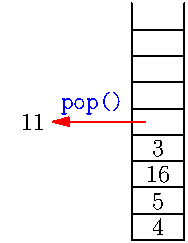
\includegraphics[height=12cm]{stack_popped}}}
    \pause \pauselevel{=7 :11}
    \put(0,0){\makebox(90,120)[br]{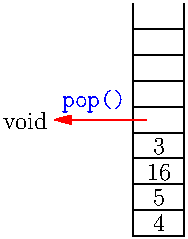
\includegraphics[height=12cm]{stack_popped_cpp}}}\pause
  \end{picture}
\end{minipage}
\end{slide}

%%%%%%%%%%%%%%%%%%%%%%% Next Slide %%%%%%%%%%%%%%%%%%%%%%%

\begin{slide}
\section{Why Use a Stack?}

\begin{PauseHighLight}
  \begin{itemize}
  \item Stacks reduces the access to memory---no longer random
    access\pause
  \item Seems counter intuitive to reduce what you can do\pause
  \item Gives you a very simple interface\pause
  \item Prevents another programmer from using memory in a way that will
    break existing code\pause
  \item Sufficient for large number of algorithms\pause
  \end{itemize}
\end{PauseHighLight}
\end{slide}

%%%%%%%%%%%%%%%%%%%%%%% Next Slide %%%%%%%%%%%%%%%%%%%%%%%

\begin{slide}
\section{Uses of Stacks}

\begin{PauseHighLight}
  \begin{itemize}
  \item Reversing an array\pause
  \item Parsing expression for compilers\pause
    \begin{itemize}
    \item balancing parentheses\pause
    \item matching XML tags\pause
    \item evaluating arithmetic expression\pause
    \end{itemize}
  \item Clustering algorithm\pause
\end{itemize}
\end{PauseHighLight}

\end{slide}

%%%%%%%%%%%%%%%%%%%%%%% Next Slide %%%%%%%%%%%%%%%%%%%%%%%

\begin{slide}
\section{Evaluating Arithmetic Expressions}

\pausebuild
\begin{center}
  \multiinclude[graphics={width=\textwidth}]{eval}  \pause
\end{center}
\end{slide}



%%%%%%%%%%%%%%%%%%%%%%% Next Slide %%%%%%%%%%%%%%%%%%%%%%%
\Outline

%%%%%%%%%%%%%%%%%%%%%%% Next Slide %%%%%%%%%%%%%%%%%%%%%%%

\begin{slide}
\section{Queues}

\pausebuild
\begin{itemize}
\item First-in-first-out (FIFO) memory model \pause
\item \jl$enqueue(elem)$\pause
\item \jl$peek()$\pauselevel{=4}\pause
\item \jl$dequeue()$\pauselevel{=6}\pause
\item C++ has a double ended queue (\jl$deque$) with
  \jl$push_front()$, \jl$push_back()$, etc.\pauselevel{=9}\pause
\end{itemize}
\begin{center}\pauselevel{=1}
  \multiinclude[graphics={width=\textwidth}]{queue}\pause
\end{center}
\end{slide}

%%%%%%%%%%%%%%%%%%%%%%% Next Slide %%%%%%%%%%%%%%%%%%%%%%%

\begin{slide}
\section{Uses of Queues}

\begin{PauseHighLight}
  \begin{itemize}
  \item Queues are heavily used in multi-threaded applications
    (e.g. operating systems)\pause
  \item Multi-threaded applications need to minimise waiting and
    ensure the integrity of the data structure (for instance when an
    exception is thrown)\pause
  \item Because of this they are more complicated than most data
    structures\pause
  \item They can be implemented using linked-lists or circular
    arrays\pause
  \end{itemize}
\end{PauseHighLight}
\end{slide}




%%%%%%%%%%%%%%%%%%%%%%% Next Slide %%%%%%%%%%%%%%%%%%%%%%%

\begin{slide}
\section{Priority Queues}

\pausebuild
\begin{itemize}
\item Queue with priorities\pause
\item \jl$insert(elem,priority)$ (in C++ \jl$push()$)\pause
\item \jl$findMin()$ (in C++ \jl$top()$)\pauselevel{=4}\pause
\item \jl$deleteMin()$ (in C++ \jl$pop()$)\pause
\end{itemize}
\begin{center}\pauselevel{=1}
  \multiinclude[graphics={width=\textwidth}]{priorityqueue}\pause
\end{center}
\end{slide}

%%%%%%%%%%%%%%%%%%%%%%% Next Slide %%%%%%%%%%%%%%%%%%%%%%%

\begin{slide}
\section{Uses of Priority Queues}

\begin{PauseHighLight}
  \begin{itemize}
  \item Queues with priorities (e.g. which threads should run)\pause
  \item Real time simulation\pause
  \item Often used in ``greedy algorithms''
    \begin{itemize}
    \item Huffman encoding
    \item Prim's minimum spanning tree algorithm\pause
    \end{itemize}
  \end{itemize}
\end{PauseHighLight}
\end{slide}


%%%%%%%%%%%%%%%%%%%%%%% Next Slide %%%%%%%%%%%%%%%%%%%%%%%

\begin{slide}
\section{Implementation of Priority Queue}

\begin{PauseHighLight}
  \begin{itemize}
  \item Could be implemented using a binary tree or linked list\pause
  \item Most efficient implementation uses a heap\pause
  \item A heap is a binary tree implemented using an array\pause
  \end{itemize}

\end{PauseHighLight}

\end{slide}


%%%%%%%%%%%%%%%%%%%%%%% Next Slide %%%%%%%%%%%%%%%%%%%%%%%
\Outline

%%%%%%%%%%%%%%%%%%%%%%% Next Slide %%%%%%%%%%%%%%%%%%%%%%%

\begin{slide}
\section{Lists}

\begin{PauseHighLight}
  \begin{itemize}
  \item In C++ the standard list is known as \jl$vector<T>$\pause
  \item That is, it is a collection where the order in which you put
    items into the list counts\pause
  \item You can have repetitions of elements\pause
  \item It has random access, e.g. \jl$v[i]$\pause
  \item You can \jl$push_back(i)$, \jl$insert$, \jl$erase$, etc.\pause
  \item C++ has a linked list class \jl$List<T>$\pause
  \end{itemize}
\end{PauseHighLight}

\end{slide}

%%%%%%%%%%%%%%%%%%%%%%% Next Slide %%%%%%%%%%%%%%%%%%%%%%%

\begin{slide}
\section{Sets}

\begin{PauseHighLight}
  \begin{itemize}
  \item Models mathematical sets\pause
  \item Container with no ordering or repetitions\pause
  \item Methods include \jl$insert$, \jl$find$, \jl$size$,
    \jl$erase$\pause
  \item Provides fast search (\jl$find$)\pause
  \item This is the class to use when you have to rapidly find whether
    an object is in the set or not\pause---don't use a list like
    \jl$vector<T>$!\pauseb
\end{itemize}  
\end{PauseHighLight}
\end{slide}

%%%%%%%%%%%%%%%%%%%%%%% Next Slide %%%%%%%%%%%%%%%%%%%%%%%

\begin{slide}
\section{Iterators}

\begin{PauseHighLight}
  \begin{itemize}
  \item Wish to act on all members of the set\pause
  \item Performed using an \jl$iterator$\pause
  \item Iterators are used by many collections\pause
  \item In C++ iterators follow the pointer convention\pause
    \begin{cpp}
      set<string> words;

      words.insert("hello");
      words.insert("world");
      
      for(auto iter = words.begin(); iter != words.end(); ++iter) {
        cout << *iter << endl;
      }
    \end{cpp}\pause
  \end{itemize}
\end{PauseHighLight}

\end{slide}

%%%%%%%%%%%%%%%%%%%%%%% Next Slide %%%%%%%%%%%%%%%%%%%%%%%

\begin{slide}
\section[-1]{Implementation of Sets}

\begin{PauseHighLight}
  \begin{itemize}
  \item Sets are very important and there are many implementations
    depending on their usage\pause
  \item Two common implementations of sets are
    \begin{itemize}
    \item hash tables: \jl$unordered_set<T>$
    \item binary trees: \jl$set<T>$ \pause
    \end{itemize}
  \item Which is most efficient depends on the application\pause
  \item Binary trees allow you to iterate in order\pause{} (iterating
    over a hash table will give you outputs in random order)\pauseb
  \item \jl$multiset<T>$ are sets with repetition\pause
  \end{itemize}
\end{PauseHighLight}
\end{slide}



%%%%%%%%%%%%%%%%%%%%%%% Next Slide %%%%%%%%%%%%%%%%%%%%%%%

\begin{slide}
\section{Maps}

\begin{PauseHighLight}
  \begin{itemize}
  \item A map provides a content addressable memory for pairs
  \textit{keyword: data}\pause
  \item It provides fast access to the data through the keyword\pause
  \item Implement as tree or hash table\pause
  \item Multimaps allows different data to be stored with the same
    keyword\pause
  \end{itemize}
\end{PauseHighLight}
\end{slide}



%%%%%%%%%%%%%%%%%%%%%%% Next Slide %%%%%%%%%%%%%%%%%%%%%%%
\Outline
%%%%%%%%%%%%%%%%%%%%%%% Next Slide %%%%%%%%%%%%%%%%%%%%%%%

\begin{slide}
\section{Connected Nodes}
\begin{minipage}{0.5\linewidth}
\vfill
\includegraphics[width=\linewidth]{clustering}
\vfill
\end{minipage}\hfil%
\begin{minipage}{0.45\linewidth}
\begin{PauseHighLight}
  \begin{itemize}
  \item A frequent problem is to find clusters of connected cells\pause
  \item Applications in computer vision, computer go, graph
    connectedness, \ldots\pause
  \end{itemize}
\end{PauseHighLight}

\end{minipage}

\end{slide}


%%%%%%%%%%%%%%%%%%%%%%% Next Slide %%%%%%%%%%%%%%%%%%%%%%%

\begin{slide}
\section[-2]{Connected Nodes}

\pb
\pause
\begin{center}
  \includegraphics[width=\linewidth]{clustering0}\mypl{1}
  \multido{\ia=1+1,\ib=2+1}{16}{%
    \llap{\includegraphics[width=\linewidth]{clustering\ia}}\mypl{\ib}}
\end{center}

\end{slide}

%%%%%%%%%%%%%%%%%%%%%%% Next Slide %%%%%%%%%%%%%%%%%%%%%%%

\begin{slide}
\section[-1]{Connected Node Algorithm}

\begin{java}
set<Node> findCluster(Node startNode, Graph graph)$\pause$
{
  stack<Node> uncheckedNodes = new Stack<Node>();
  set<Node> clusterNodes = new HashSet<Node>();$\pause$

  uncheckedNodes.push(startNode);
  clusterNodes.add(startNode);$\pause$

  while (!uncheckedNodes.empty()) {$\pause$
    Node next = uncheckedNodes.top();   uncheckedNodes.pop();
    vector<Node> neighbours = graph.getNeighbours(next);$\pause$
    for (Node neigh: neighbours) {
      if (graph.isOccupied(neigh) && !clusterNodes.contains(neigh) ) {
        uncheckedNodes.push(neigh);
        clusterNodes.insert(neigh);
      }
    }$\pause$
  }

  return clusterNodes;
}$\pause$
\end{java}
\end{slide}


%%%%%%%%%%%%%%%%%%%%%%% Next Slide %%%%%%%%%%%%%%%%%%%%%%%

\begin{slide}
\section{Lessons}

\begin{PauseHighLight}
  \begin{itemize}
  \item Abstract Data Types (ADT) are interfaces to data\pause
  \item Their purpose is to allow the programmer to declare their
    intentions\pause
  \item They often have different implementations with different
    properties\pause
  \item The most efficient implementation is not always
    obvious\pause---we will see many of these implementations as we go
    through this course\pause
  \item You need to know the common ADTs (e.g. Stack, Queue, List, Set,
    Map) and how and when to use them\pause
  \end{itemize}
\end{PauseHighLight}
\end{slide}

